\documentclass[twoside]{book}

% Packages required by doxygen
\usepackage{fixltx2e}
\usepackage{calc}
\usepackage{doxygen}
\usepackage[export]{adjustbox} % also loads graphicx
\usepackage{graphicx}
\usepackage[utf8]{inputenc}
\usepackage{makeidx}
\usepackage{multicol}
\usepackage{multirow}
\PassOptionsToPackage{warn}{textcomp}
\usepackage{textcomp}
\usepackage[nointegrals]{wasysym}
\usepackage[table]{xcolor}

% NLS support packages
\usepackage[french]{babel}

% Font selection
\usepackage[T1]{fontenc}
\usepackage[scaled=.90]{helvet}
\usepackage{courier}
\usepackage{amssymb}
\usepackage{sectsty}
\renewcommand{\familydefault}{\sfdefault}
\allsectionsfont{%
  \fontseries{bc}\selectfont%
  \color{darkgray}%
}
\renewcommand{\DoxyLabelFont}{%
  \fontseries{bc}\selectfont%
  \color{darkgray}%
}
\newcommand{\+}{\discretionary{\mbox{\scriptsize$\hookleftarrow$}}{}{}}

% Page & text layout
\usepackage{geometry}
\geometry{%
  a4paper,%
  top=2.5cm,%
  bottom=2.5cm,%
  left=2.5cm,%
  right=2.5cm%
}
\tolerance=750
\hfuzz=15pt
\hbadness=750
\setlength{\emergencystretch}{15pt}
\setlength{\parindent}{0cm}
\setlength{\parskip}{3ex plus 2ex minus 2ex}
\makeatletter
\renewcommand{\paragraph}{%
  \@startsection{paragraph}{4}{0ex}{-1.0ex}{1.0ex}{%
    \normalfont\normalsize\bfseries\SS@parafont%
  }%
}
\renewcommand{\subparagraph}{%
  \@startsection{subparagraph}{5}{0ex}{-1.0ex}{1.0ex}{%
    \normalfont\normalsize\bfseries\SS@subparafont%
  }%
}
\makeatother

% Headers & footers
\usepackage{fancyhdr}
\pagestyle{fancyplain}
\fancyhead[LE]{\fancyplain{}{\bfseries\thepage}}
\fancyhead[CE]{\fancyplain{}{}}
\fancyhead[RE]{\fancyplain{}{\bfseries\leftmark}}
\fancyhead[LO]{\fancyplain{}{\bfseries\rightmark}}
\fancyhead[CO]{\fancyplain{}{}}
\fancyhead[RO]{\fancyplain{}{\bfseries\thepage}}
\fancyfoot[LE]{\fancyplain{}{}}
\fancyfoot[CE]{\fancyplain{}{}}
\fancyfoot[RE]{\fancyplain{}{\bfseries\scriptsize Généré par Doxygen }}
\fancyfoot[LO]{\fancyplain{}{\bfseries\scriptsize Généré par Doxygen }}
\fancyfoot[CO]{\fancyplain{}{}}
\fancyfoot[RO]{\fancyplain{}{}}
\renewcommand{\footrulewidth}{0.4pt}
\renewcommand{\chaptermark}[1]{%
  \markboth{#1}{}%
}
\renewcommand{\sectionmark}[1]{%
  \markright{\thesection\ #1}%
}

% Indices & bibliography
\usepackage{natbib}
\usepackage[titles]{tocloft}
\setcounter{tocdepth}{3}
\setcounter{secnumdepth}{5}
\makeindex

% Hyperlinks (required, but should be loaded last)
\usepackage{ifpdf}
\ifpdf
  \usepackage[pdftex,pagebackref=true]{hyperref}
\else
  \usepackage[ps2pdf,pagebackref=true]{hyperref}
\fi
\hypersetup{%
  colorlinks=true,%
  linkcolor=blue,%
  citecolor=blue,%
  unicode%
}

% Custom commands
\newcommand{\clearemptydoublepage}{%
  \newpage{\pagestyle{empty}\cleardoublepage}%
}

\usepackage{caption}
\captionsetup{labelsep=space,justification=centering,font={bf},singlelinecheck=off,skip=4pt,position=top}

%===== C O N T E N T S =====

\begin{document}

% Titlepage & ToC
\hypersetup{pageanchor=false,
             bookmarksnumbered=true,
             pdfencoding=unicode
            }
\pagenumbering{roman}
\begin{titlepage}
\vspace*{7cm}
\begin{center}%
{\Large Enigme\+\_\+2 \\[1ex]\large 1 }\\
\vspace*{1cm}
{\large Généré par Doxygen 1.8.11}\\
\end{center}
\end{titlepage}
\clearemptydoublepage
\tableofcontents
\clearemptydoublepage
\pagenumbering{arabic}
\hypersetup{pageanchor=true}

%--- Begin generated contents ---
\chapter{Index des structures de données}
\section{Structures de données}
Liste des structures de données avec une brève description \+:\begin{DoxyCompactList}
\item\contentsline{section}{\hyperlink{structText}{Text} \\*Struct for \hyperlink{structText}{Text} }{\pageref{structText}}{}
\end{DoxyCompactList}

\chapter{Index des fichiers}
\section{Liste des fichiers}
Liste de tous les fichiers avec une brève description \+:\begin{DoxyCompactList}
\item\contentsline{section}{\hyperlink{enigme__clavier_8c}{enigme\+\_\+clavier.\+c} \\*Writing Program }{\pageref{enigme__clavier_8c}}{}
\item\contentsline{section}{\hyperlink{enigme__clavier_8h}{enigme\+\_\+clavier.\+h} }{\pageref{enigme__clavier_8h}}{}
\item\contentsline{section}{\hyperlink{main_8c}{main.\+c} \\*Testing Program }{\pageref{main_8c}}{}
\end{DoxyCompactList}

\chapter{Documentation des structures de données}
\hypertarget{structText}{}\section{Référence de la structure Text}
\label{structText}\index{Text@{Text}}


struct for \hyperlink{structText}{Text}  




{\ttfamily \#include $<$text.\+h$>$}

\subsection*{Champs de données}
\begin{DoxyCompactItemize}
\item 
S\+D\+L\+\_\+\+Surface $\ast$ \hyperlink{structText_aff6d6c980d60246e053f3073f52b6176}{score}
\item 
S\+D\+L\+\_\+\+Surface $\ast$ \hyperlink{structText_a0fcc09b9e71277a628a94d5cc1009e82}{vie}
\item 
S\+D\+L\+\_\+\+Surface $\ast$ \hyperlink{structText_acb7a71b616bd8ff9c3bf1ed75b7075aa}{tmp}
\end{DoxyCompactItemize}


\subsection{Description détaillée}
struct for \hyperlink{structText}{Text} 

\subsection{Documentation des champs}
\index{Text@{Text}!score@{score}}
\index{score@{score}!Text@{Text}}
\subsubsection[{\texorpdfstring{score}{score}}]{\setlength{\rightskip}{0pt plus 5cm}S\+D\+L\+\_\+\+Surface$\ast$ Text\+::score}\hypertarget{structText_aff6d6c980d60246e053f3073f52b6176}{}\label{structText_aff6d6c980d60246e053f3073f52b6176}
Score \index{Text@{Text}!tmp@{tmp}}
\index{tmp@{tmp}!Text@{Text}}
\subsubsection[{\texorpdfstring{tmp}{tmp}}]{\setlength{\rightskip}{0pt plus 5cm}S\+D\+L\+\_\+\+Surface$\ast$ Text\+::tmp}\hypertarget{structText_acb7a71b616bd8ff9c3bf1ed75b7075aa}{}\label{structText_acb7a71b616bd8ff9c3bf1ed75b7075aa}
Temps jeu \index{Text@{Text}!vie@{vie}}
\index{vie@{vie}!Text@{Text}}
\subsubsection[{\texorpdfstring{vie}{vie}}]{\setlength{\rightskip}{0pt plus 5cm}S\+D\+L\+\_\+\+Surface$\ast$ Text\+::vie}\hypertarget{structText_a0fcc09b9e71277a628a94d5cc1009e82}{}\label{structText_a0fcc09b9e71277a628a94d5cc1009e82}
Vie 

La documentation de cette structure a été générée à partir du fichier suivant \+:\begin{DoxyCompactItemize}
\item 
\hyperlink{text_8h}{text.\+h}\end{DoxyCompactItemize}

\chapter{Documentation des fichiers}
\hypertarget{defs_8h}{}\section{Référence du fichier defs.\+h}
\label{defs_8h}\index{defs.\+h@{defs.\+h}}
Ce graphe montre quels fichiers incluent directement ou indirectement ce fichier \+:
\nopagebreak
\begin{figure}[H]
\begin{center}
\leavevmode
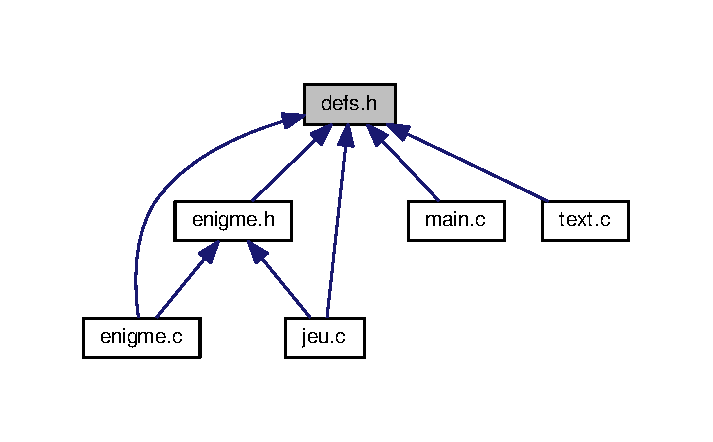
\includegraphics[width=342pt]{defs_8h__dep__incl}
\end{center}
\end{figure}
\subsection*{Macros}
\begin{DoxyCompactItemize}
\item 
\#define \hyperlink{defs_8h_a9b6bc9242882d1e758e06ed751a2e8ec}{S\+C\+R\+E\+E\+N\+\_\+W}~1100
\item 
\#define \hyperlink{defs_8h_a27cddfd509d28b4b2b0b44c093fac090}{S\+C\+R\+E\+E\+N\+\_\+H}~700
\end{DoxyCompactItemize}
\subsection*{Définitions de type}
\begin{DoxyCompactItemize}
\item 
typedef int \hyperlink{defs_8h_a1062901a7428fdd9c7f180f5e01ea056}{bool}
\end{DoxyCompactItemize}


\subsection{Documentation des macros}
\index{defs.\+h@{defs.\+h}!S\+C\+R\+E\+E\+N\+\_\+H@{S\+C\+R\+E\+E\+N\+\_\+H}}
\index{S\+C\+R\+E\+E\+N\+\_\+H@{S\+C\+R\+E\+E\+N\+\_\+H}!defs.\+h@{defs.\+h}}
\subsubsection[{\texorpdfstring{S\+C\+R\+E\+E\+N\+\_\+H}{SCREEN_H}}]{\setlength{\rightskip}{0pt plus 5cm}\#define S\+C\+R\+E\+E\+N\+\_\+H~700}\hypertarget{defs_8h_a27cddfd509d28b4b2b0b44c093fac090}{}\label{defs_8h_a27cddfd509d28b4b2b0b44c093fac090}
\index{defs.\+h@{defs.\+h}!S\+C\+R\+E\+E\+N\+\_\+W@{S\+C\+R\+E\+E\+N\+\_\+W}}
\index{S\+C\+R\+E\+E\+N\+\_\+W@{S\+C\+R\+E\+E\+N\+\_\+W}!defs.\+h@{defs.\+h}}
\subsubsection[{\texorpdfstring{S\+C\+R\+E\+E\+N\+\_\+W}{SCREEN_W}}]{\setlength{\rightskip}{0pt plus 5cm}\#define S\+C\+R\+E\+E\+N\+\_\+W~1100}\hypertarget{defs_8h_a9b6bc9242882d1e758e06ed751a2e8ec}{}\label{defs_8h_a9b6bc9242882d1e758e06ed751a2e8ec}


\subsection{Documentation des définitions de type}
\index{defs.\+h@{defs.\+h}!bool@{bool}}
\index{bool@{bool}!defs.\+h@{defs.\+h}}
\subsubsection[{\texorpdfstring{bool}{bool}}]{\setlength{\rightskip}{0pt plus 5cm}typedef int {\bf bool}}\hypertarget{defs_8h_a1062901a7428fdd9c7f180f5e01ea056}{}\label{defs_8h_a1062901a7428fdd9c7f180f5e01ea056}

\hypertarget{enigme_8c}{}\section{Référence du fichier enigme.\+c}
\label{enigme_8c}\index{enigme.\+c@{enigme.\+c}}


Writing Program.  


{\ttfamily \#include $<$stdio.\+h$>$}\\*
{\ttfamily \#include $<$stdlib.\+h$>$}\\*
{\ttfamily \#include $<$S\+D\+L/\+S\+D\+L.\+h$>$}\\*
{\ttfamily \#include $<$S\+D\+L/\+S\+D\+L\+\_\+image.\+h$>$}\\*
{\ttfamily \#include $<$S\+D\+L/\+S\+D\+L\+\_\+mixer.\+h$>$}\\*
{\ttfamily \#include \char`\"{}enigme.\+h\char`\"{}}\\*
{\ttfamily \#include \char`\"{}random.\+h\char`\"{}}\\*
{\ttfamily \#include \char`\"{}defs.\+h\char`\"{}}\\*
{\ttfamily \#include \char`\"{}jeu.\+h\char`\"{}}\\*
{\ttfamily \#include \char`\"{}text.\+h\char`\"{}}\\*
Graphe des dépendances par inclusion de enigme.\+c\+:\nopagebreak
\begin{figure}[H]
\begin{center}
\leavevmode
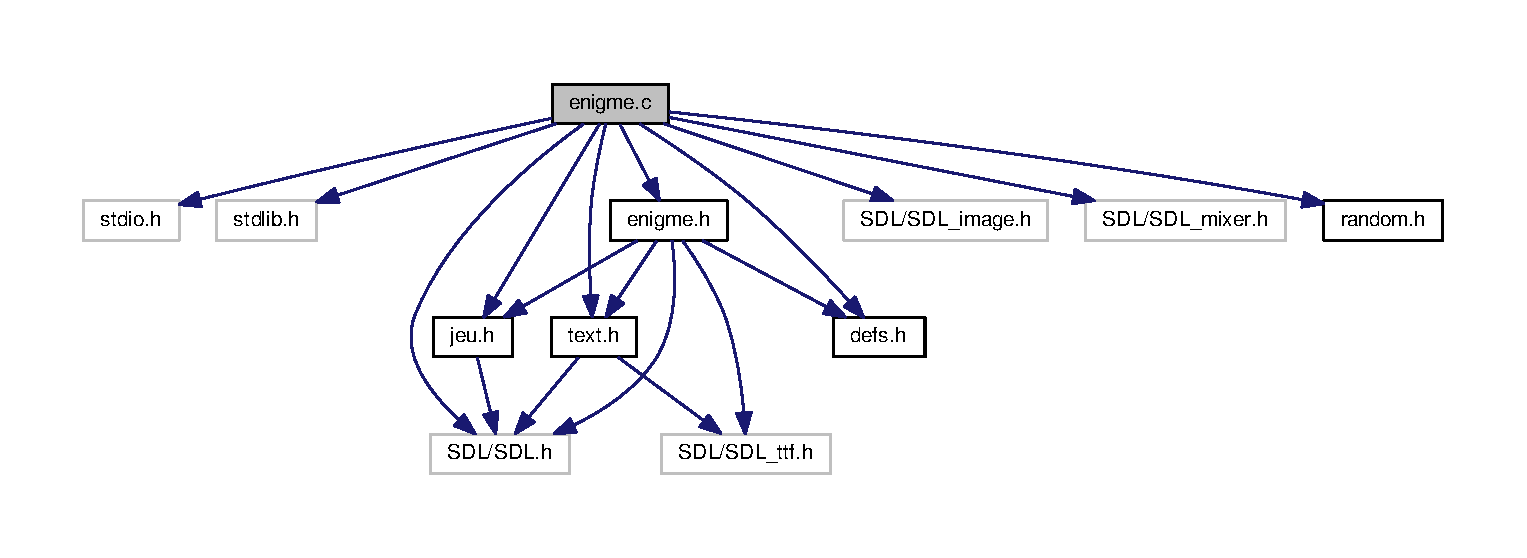
\includegraphics[width=350pt]{enigme_8c__incl}
\end{center}
\end{figure}
\subsection*{Fonctions}
\begin{DoxyCompactItemize}
\item 
int \hyperlink{enigme_8c_af3c9a532bad2669db67b723315a40e2a}{enigme} (S\+D\+L\+\_\+\+Surface $\ast$screen, T\+T\+F\+\_\+\+Font $\ast$police, \hyperlink{structText}{Text} $\ast$T, int $\ast$vie, int $\ast$score, int $\ast$tmp)
\begin{DoxyCompactList}\small\item\em Ecriture de la fonction enigme(affichage et resolution) \end{DoxyCompactList}\end{DoxyCompactItemize}


\subsection{Description détaillée}
Writing Program. 

\begin{DoxyAuthor}{Auteur}
Mintoua T Level-\/\+Up 
\end{DoxyAuthor}
\begin{DoxyVersion}{Version}
0.\+1 
\end{DoxyVersion}
\begin{DoxyDate}{Date}
Apr 21, 2019
\end{DoxyDate}
Writing program for enigme 

\subsection{Documentation des fonctions}
\index{enigme.\+c@{enigme.\+c}!enigme@{enigme}}
\index{enigme@{enigme}!enigme.\+c@{enigme.\+c}}
\subsubsection[{\texorpdfstring{enigme(\+S\+D\+L\+\_\+\+Surface $\ast$screen, T\+T\+F\+\_\+\+Font $\ast$police, Text $\ast$\+T, int $\ast$vie, int $\ast$score, int $\ast$tmp)}{enigme(SDL_Surface *screen, TTF_Font *police, Text *T, int *vie, int *score, int *tmp)}}]{\setlength{\rightskip}{0pt plus 5cm}int enigme (
\begin{DoxyParamCaption}
\item[{S\+D\+L\+\_\+\+Surface $\ast$}]{screen, }
\item[{T\+T\+F\+\_\+\+Font $\ast$}]{police, }
\item[{{\bf Text} $\ast$}]{T, }
\item[{int $\ast$}]{vie, }
\item[{int $\ast$}]{score, }
\item[{int $\ast$}]{tmp}
\end{DoxyParamCaption}
)}\hypertarget{enigme_8c_af3c9a532bad2669db67b723315a40e2a}{}\label{enigme_8c_af3c9a532bad2669db67b723315a40e2a}


Ecriture de la fonction enigme(affichage et resolution) 

\begin{DoxyAuthor}{Auteur}
Mintoua T Level-\/\+Up 
\end{DoxyAuthor}

\begin{DoxyParams}{Paramètres}
{\em screen} & .c\textquotesingle{}est l\textquotesingle{}écran du jeu \\
\hline
{\em police} & .La police des textes \\
\hline
{\em T} & .Le texte ecrit \\
\hline
{\em vie} & .La vie du joueur \\
\hline
{\em score} & .Son score \\
\hline
{\em tmp} & .Le temps du jeu \\
\hline
\end{DoxyParams}
\begin{DoxyDate}{Date}
Apr 28, 2019 
\end{DoxyDate}
\begin{DoxyReturn}{Renvoie}
1 pour vraie 0 pour fausse reponse 
\end{DoxyReturn}


Voici le graphe d\textquotesingle{}appel pour cette fonction \+:
\nopagebreak
\begin{figure}[H]
\begin{center}
\leavevmode
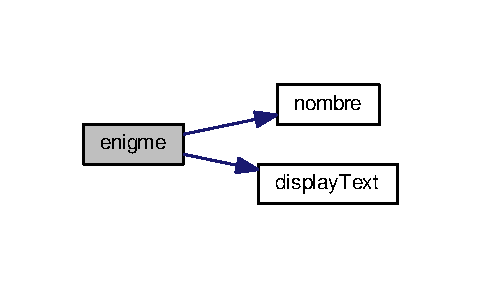
\includegraphics[width=231pt]{enigme_8c_af3c9a532bad2669db67b723315a40e2a_cgraph}
\end{center}
\end{figure}




Voici le graphe des appelants de cette fonction \+:
\nopagebreak
\begin{figure}[H]
\begin{center}
\leavevmode
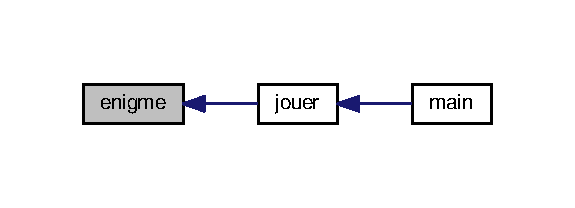
\includegraphics[width=276pt]{enigme_8c_af3c9a532bad2669db67b723315a40e2a_icgraph}
\end{center}
\end{figure}



\hypertarget{enigme_8h}{}\section{Référence du fichier enigme.\+h}
\label{enigme_8h}\index{enigme.\+h@{enigme.\+h}}
{\ttfamily \#include $<$S\+D\+L/\+S\+D\+L.\+h$>$}\\*
{\ttfamily \#include $<$S\+D\+L/\+S\+D\+L\+\_\+ttf.\+h$>$}\\*
{\ttfamily \#include \char`\"{}defs.\+h\char`\"{}}\\*
{\ttfamily \#include \char`\"{}jeu.\+h\char`\"{}}\\*
{\ttfamily \#include \char`\"{}text.\+h\char`\"{}}\\*
Graphe des dépendances par inclusion de enigme.\+h\+:\nopagebreak
\begin{figure}[H]
\begin{center}
\leavevmode
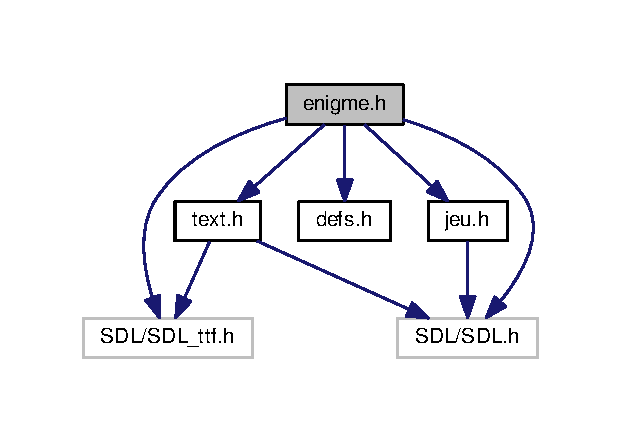
\includegraphics[width=298pt]{enigme_8h__incl}
\end{center}
\end{figure}
Ce graphe montre quels fichiers incluent directement ou indirectement ce fichier \+:
\nopagebreak
\begin{figure}[H]
\begin{center}
\leavevmode
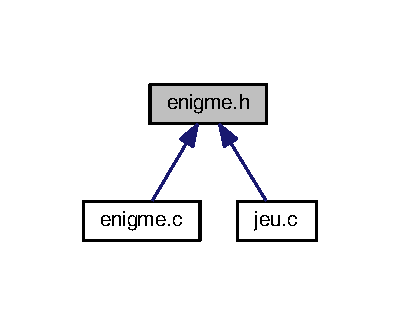
\includegraphics[width=192pt]{enigme_8h__dep__incl}
\end{center}
\end{figure}
\subsection*{Fonctions}
\begin{DoxyCompactItemize}
\item 
int \hyperlink{enigme_8h_af3c9a532bad2669db67b723315a40e2a}{enigme} (S\+D\+L\+\_\+\+Surface $\ast$screen, T\+T\+F\+\_\+\+Font $\ast$police, \hyperlink{structText}{Text} $\ast$T, int $\ast$vie, int $\ast$score, int $\ast$tmp)
\begin{DoxyCompactList}\small\item\em Ecriture de la fonction enigme(affichage et resolution) \end{DoxyCompactList}\end{DoxyCompactItemize}


\subsection{Documentation des fonctions}
\index{enigme.\+h@{enigme.\+h}!enigme@{enigme}}
\index{enigme@{enigme}!enigme.\+h@{enigme.\+h}}
\subsubsection[{\texorpdfstring{enigme(\+S\+D\+L\+\_\+\+Surface $\ast$screen, T\+T\+F\+\_\+\+Font $\ast$police, Text $\ast$\+T, int $\ast$vie, int $\ast$score, int $\ast$tmp)}{enigme(SDL_Surface *screen, TTF_Font *police, Text *T, int *vie, int *score, int *tmp)}}]{\setlength{\rightskip}{0pt plus 5cm}int enigme (
\begin{DoxyParamCaption}
\item[{S\+D\+L\+\_\+\+Surface $\ast$}]{screen, }
\item[{T\+T\+F\+\_\+\+Font $\ast$}]{police, }
\item[{{\bf Text} $\ast$}]{T, }
\item[{int $\ast$}]{vie, }
\item[{int $\ast$}]{score, }
\item[{int $\ast$}]{tmp}
\end{DoxyParamCaption}
)}\hypertarget{enigme_8h_af3c9a532bad2669db67b723315a40e2a}{}\label{enigme_8h_af3c9a532bad2669db67b723315a40e2a}


Ecriture de la fonction enigme(affichage et resolution) 

\begin{DoxyAuthor}{Auteur}
Mintoua T Level-\/\+Up 
\end{DoxyAuthor}

\begin{DoxyParams}{Paramètres}
{\em screen} & .c\textquotesingle{}est l\textquotesingle{}écran du jeu \\
\hline
{\em police} & .La police des textes \\
\hline
{\em T} & .Le texte ecrit \\
\hline
{\em vie} & .La vie du joueur \\
\hline
{\em score} & .Son score \\
\hline
{\em tmp} & .Le temps du jeu \\
\hline
\end{DoxyParams}
\begin{DoxyDate}{Date}
Apr 28, 2019 
\end{DoxyDate}
\begin{DoxyReturn}{Renvoie}
1 pour vraie 0 pour fausse reponse 
\end{DoxyReturn}


Voici le graphe d\textquotesingle{}appel pour cette fonction \+:
\nopagebreak
\begin{figure}[H]
\begin{center}
\leavevmode
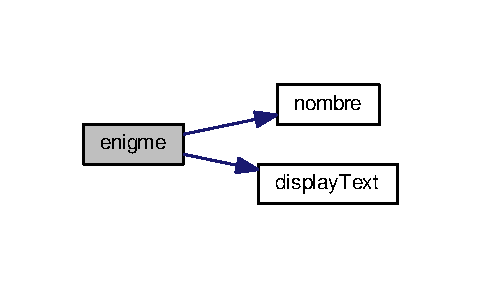
\includegraphics[width=231pt]{enigme_8h_af3c9a532bad2669db67b723315a40e2a_cgraph}
\end{center}
\end{figure}




Voici le graphe des appelants de cette fonction \+:
\nopagebreak
\begin{figure}[H]
\begin{center}
\leavevmode
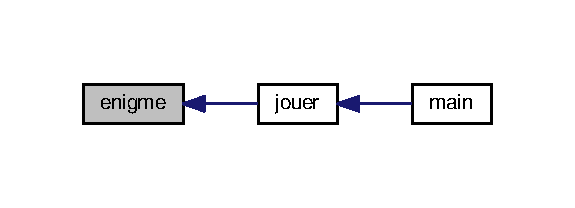
\includegraphics[width=276pt]{enigme_8h_af3c9a532bad2669db67b723315a40e2a_icgraph}
\end{center}
\end{figure}



\hypertarget{jeu_8c}{}\section{Référence du fichier jeu.\+c}
\label{jeu_8c}\index{jeu.\+c@{jeu.\+c}}


Writing Program.  


{\ttfamily \#include $<$S\+D\+L/\+S\+D\+L.\+h$>$}\\*
{\ttfamily \#include $<$S\+D\+L/\+S\+D\+L\+\_\+image.\+h$>$}\\*
{\ttfamily \#include $<$S\+D\+L/\+S\+D\+L\+\_\+ttf.\+h$>$}\\*
{\ttfamily \#include \char`\"{}defs.\+h\char`\"{}}\\*
{\ttfamily \#include \char`\"{}jeu.\+h\char`\"{}}\\*
{\ttfamily \#include \char`\"{}text.\+h\char`\"{}}\\*
{\ttfamily \#include \char`\"{}enigme.\+h\char`\"{}}\\*
Graphe des dépendances par inclusion de jeu.\+c\+:\nopagebreak
\begin{figure}[H]
\begin{center}
\leavevmode
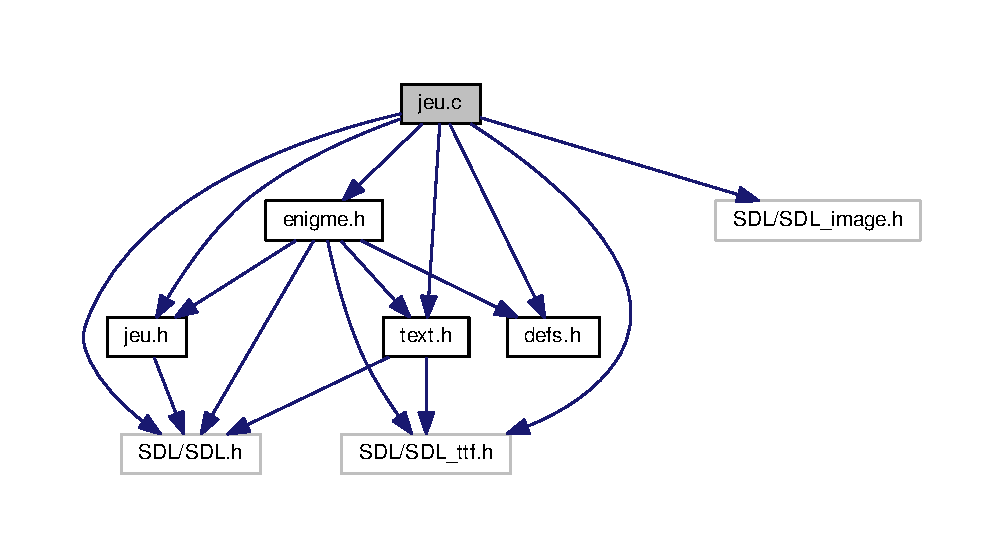
\includegraphics[width=350pt]{jeu_8c__incl}
\end{center}
\end{figure}
\subsection*{Fonctions}
\begin{DoxyCompactItemize}
\item 
int \hyperlink{jeu_8c_ad9c436fc5815440f57648231b18e2caf}{jouer} (S\+D\+L\+\_\+\+Surface $\ast$screen)
\begin{DoxyCompactList}\small\item\em Pour Afficher le jeu. \end{DoxyCompactList}\end{DoxyCompactItemize}


\subsection{Description détaillée}
Writing Program. 

\begin{DoxyAuthor}{Auteur}
Mintoua T Level-\/\+Up 
\end{DoxyAuthor}
\begin{DoxyVersion}{Version}
0.\+1 
\end{DoxyVersion}
\begin{DoxyDate}{Date}
Apr 28, 2019
\end{DoxyDate}
Writing program for enigme 

\subsection{Documentation des fonctions}
\index{jeu.\+c@{jeu.\+c}!jouer@{jouer}}
\index{jouer@{jouer}!jeu.\+c@{jeu.\+c}}
\subsubsection[{\texorpdfstring{jouer(\+S\+D\+L\+\_\+\+Surface $\ast$screen)}{jouer(SDL_Surface *screen)}}]{\setlength{\rightskip}{0pt plus 5cm}int jouer (
\begin{DoxyParamCaption}
\item[{S\+D\+L\+\_\+\+Surface $\ast$}]{screen}
\end{DoxyParamCaption}
)}\hypertarget{jeu_8c_ad9c436fc5815440f57648231b18e2caf}{}\label{jeu_8c_ad9c436fc5815440f57648231b18e2caf}


Pour Afficher le jeu. 

\begin{DoxyAuthor}{Auteur}
Mintoua T Level-\/\+Up 
\end{DoxyAuthor}

\begin{DoxyParams}{Paramètres}
{\em screen} & .c\textquotesingle{}est l\textquotesingle{}écran du jeu \\
\hline
\end{DoxyParams}
\begin{DoxyDate}{Date}
Apr 28, 2019 
\end{DoxyDate}
\begin{DoxyReturn}{Renvoie}
1 bon jeu ou 0 fin jeu 
\end{DoxyReturn}


Voici le graphe d\textquotesingle{}appel pour cette fonction \+:
\nopagebreak
\begin{figure}[H]
\begin{center}
\leavevmode
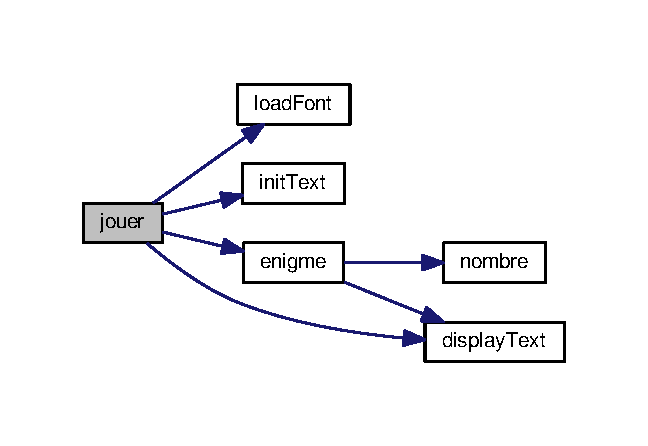
\includegraphics[width=311pt]{jeu_8c_ad9c436fc5815440f57648231b18e2caf_cgraph}
\end{center}
\end{figure}




Voici le graphe des appelants de cette fonction \+:\nopagebreak
\begin{figure}[H]
\begin{center}
\leavevmode
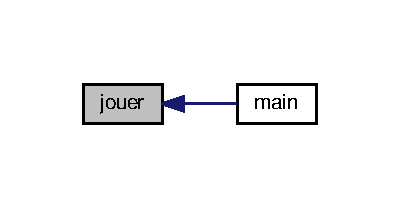
\includegraphics[width=192pt]{jeu_8c_ad9c436fc5815440f57648231b18e2caf_icgraph}
\end{center}
\end{figure}



\hypertarget{jeu_8h}{}\section{Référence du fichier jeu.\+h}
\label{jeu_8h}\index{jeu.\+h@{jeu.\+h}}
{\ttfamily \#include $<$S\+D\+L/\+S\+D\+L.\+h$>$}\\*
Graphe des dépendances par inclusion de jeu.\+h\+:\nopagebreak
\begin{figure}[H]
\begin{center}
\leavevmode
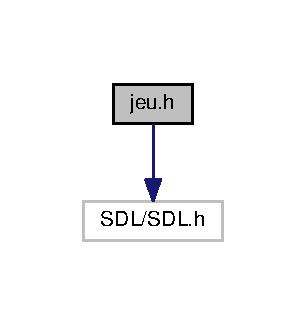
\includegraphics[width=147pt]{jeu_8h__incl}
\end{center}
\end{figure}
Ce graphe montre quels fichiers incluent directement ou indirectement ce fichier \+:
\nopagebreak
\begin{figure}[H]
\begin{center}
\leavevmode
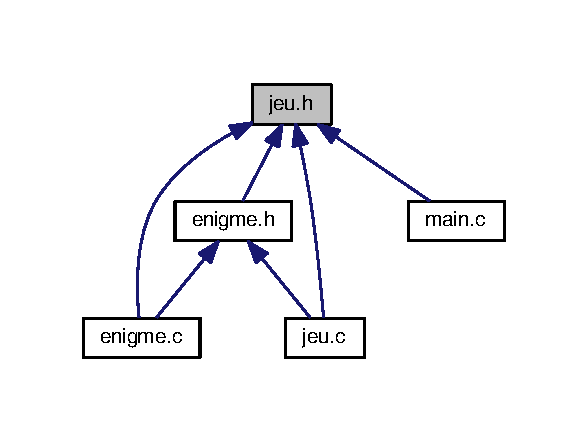
\includegraphics[width=282pt]{jeu_8h__dep__incl}
\end{center}
\end{figure}
\subsection*{Fonctions}
\begin{DoxyCompactItemize}
\item 
int \hyperlink{jeu_8h_ad9c436fc5815440f57648231b18e2caf}{jouer} (S\+D\+L\+\_\+\+Surface $\ast$screen)
\begin{DoxyCompactList}\small\item\em Pour Afficher le jeu. \end{DoxyCompactList}\end{DoxyCompactItemize}


\subsection{Documentation des fonctions}
\index{jeu.\+h@{jeu.\+h}!jouer@{jouer}}
\index{jouer@{jouer}!jeu.\+h@{jeu.\+h}}
\subsubsection[{\texorpdfstring{jouer(\+S\+D\+L\+\_\+\+Surface $\ast$screen)}{jouer(SDL_Surface *screen)}}]{\setlength{\rightskip}{0pt plus 5cm}int jouer (
\begin{DoxyParamCaption}
\item[{S\+D\+L\+\_\+\+Surface $\ast$}]{screen}
\end{DoxyParamCaption}
)}\hypertarget{jeu_8h_ad9c436fc5815440f57648231b18e2caf}{}\label{jeu_8h_ad9c436fc5815440f57648231b18e2caf}


Pour Afficher le jeu. 

\begin{DoxyAuthor}{Auteur}
Mintoua T Level-\/\+Up 
\end{DoxyAuthor}

\begin{DoxyParams}{Paramètres}
{\em screen} & .c\textquotesingle{}est l\textquotesingle{}écran du jeu \\
\hline
\end{DoxyParams}
\begin{DoxyDate}{Date}
Apr 28, 2019 
\end{DoxyDate}
\begin{DoxyReturn}{Renvoie}
1 bon jeu ou 0 fin jeu 
\end{DoxyReturn}


Voici le graphe d\textquotesingle{}appel pour cette fonction \+:
\nopagebreak
\begin{figure}[H]
\begin{center}
\leavevmode
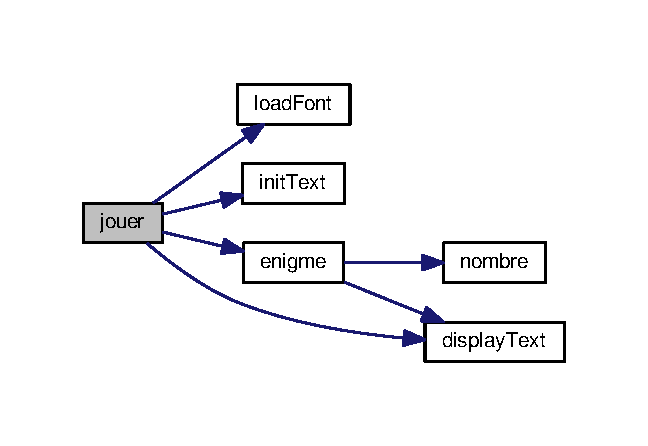
\includegraphics[width=311pt]{jeu_8h_ad9c436fc5815440f57648231b18e2caf_cgraph}
\end{center}
\end{figure}




Voici le graphe des appelants de cette fonction \+:\nopagebreak
\begin{figure}[H]
\begin{center}
\leavevmode
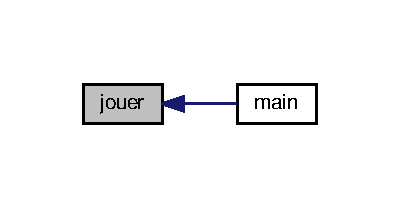
\includegraphics[width=192pt]{jeu_8h_ad9c436fc5815440f57648231b18e2caf_icgraph}
\end{center}
\end{figure}



\hypertarget{main_8c}{}\section{Référence du fichier main.\+c}
\label{main_8c}\index{main.\+c@{main.\+c}}


Testing Program.  


{\ttfamily \#include $<$stdio.\+h$>$}\\*
{\ttfamily \#include $<$stdlib.\+h$>$}\\*
{\ttfamily \#include $<$S\+D\+L/\+S\+D\+L.\+h$>$}\\*
{\ttfamily \#include $<$S\+D\+L/\+S\+D\+L\+\_\+image.\+h$>$}\\*
{\ttfamily \#include $<$S\+D\+L/\+S\+D\+L\+\_\+ttf.\+h$>$}\\*
{\ttfamily \#include $<$string.\+h$>$}\\*
{\ttfamily \#include $<$ctype.\+h$>$}\\*
{\ttfamily \#include $<$time.\+h$>$}\\*
{\ttfamily \#include \char`\"{}enigme\+\_\+clavier.\+h\char`\"{}}\\*
Graphe des dépendances par inclusion de main.\+c\+:
\nopagebreak
\begin{figure}[H]
\begin{center}
\leavevmode
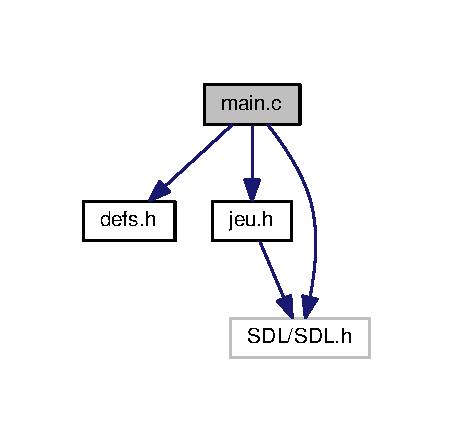
\includegraphics[width=350pt]{main_8c__incl}
\end{center}
\end{figure}
\subsection*{Fonctions}
\begin{DoxyCompactItemize}
\item 
int \hyperlink{main_8c_ae66f6b31b5ad750f1fe042a706a4e3d4}{main} ()
\end{DoxyCompactItemize}


\subsection{Description détaillée}
Testing Program. 

\begin{DoxyAuthor}{Auteur}
Mintoua T Level-\/\+Up 
\end{DoxyAuthor}
\begin{DoxyVersion}{Version}
0.\+1 
\end{DoxyVersion}
\begin{DoxyDate}{Date}
Apr 21, 2019
\end{DoxyDate}
Testing program for enigme 

\subsection{Documentation des fonctions}
\index{main.\+c@{main.\+c}!main@{main}}
\index{main@{main}!main.\+c@{main.\+c}}
\subsubsection[{\texorpdfstring{main()}{main()}}]{\setlength{\rightskip}{0pt plus 5cm}int main (
\begin{DoxyParamCaption}
{}
\end{DoxyParamCaption}
)}\hypertarget{main_8c_ae66f6b31b5ad750f1fe042a706a4e3d4}{}\label{main_8c_ae66f6b31b5ad750f1fe042a706a4e3d4}


Voici le graphe d\textquotesingle{}appel pour cette fonction \+:
\nopagebreak
\begin{figure}[H]
\begin{center}
\leavevmode
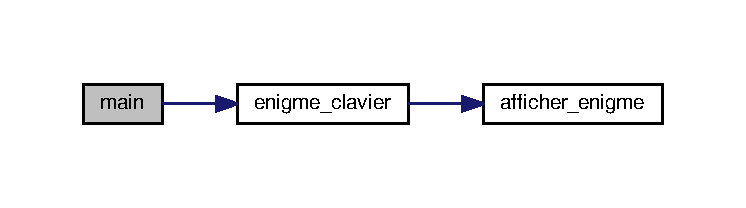
\includegraphics[width=350pt]{main_8c_ae66f6b31b5ad750f1fe042a706a4e3d4_cgraph}
\end{center}
\end{figure}



\hypertarget{random_8c}{}\section{Référence du fichier random.\+c}
\label{random_8c}\index{random.\+c@{random.\+c}}


Writing Program.  


{\ttfamily \#include $<$stdio.\+h$>$}\\*
{\ttfamily \#include $<$stdlib.\+h$>$}\\*
{\ttfamily \#include $<$time.\+h$>$}\\*
{\ttfamily \#include \char`\"{}random.\+h\char`\"{}}\\*
Graphe des dépendances par inclusion de random.\+c\+:\nopagebreak
\begin{figure}[H]
\begin{center}
\leavevmode
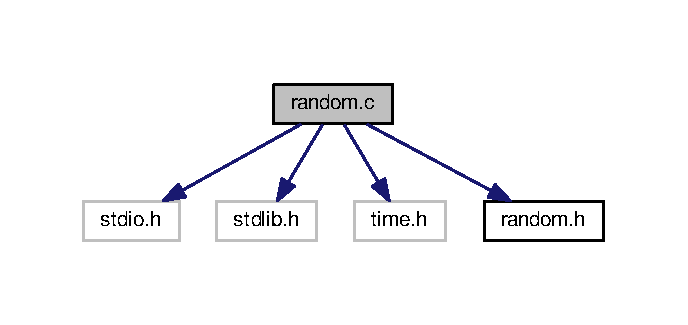
\includegraphics[width=330pt]{random_8c__incl}
\end{center}
\end{figure}
\subsection*{Fonctions}
\begin{DoxyCompactItemize}
\item 
int \hyperlink{random_8c_a61c7a4ac34762307c8ad873e71774a43}{nombre} (void)
\begin{DoxyCompactList}\small\item\em Pour calculer un nbre aleatoire. \end{DoxyCompactList}\end{DoxyCompactItemize}


\subsection{Description détaillée}
Writing Program. 

\begin{DoxyAuthor}{Auteur}
Mintoua T Level-\/\+Up 
\end{DoxyAuthor}
\begin{DoxyVersion}{Version}
0.\+1 
\end{DoxyVersion}
\begin{DoxyDate}{Date}
Apr 28, 2019
\end{DoxyDate}
Writing program for Random 

\subsection{Documentation des fonctions}
\index{random.\+c@{random.\+c}!nombre@{nombre}}
\index{nombre@{nombre}!random.\+c@{random.\+c}}
\subsubsection[{\texorpdfstring{nombre(void)}{nombre(void)}}]{\setlength{\rightskip}{0pt plus 5cm}int nombre (
\begin{DoxyParamCaption}
\item[{void}]{}
\end{DoxyParamCaption}
)}\hypertarget{random_8c_a61c7a4ac34762307c8ad873e71774a43}{}\label{random_8c_a61c7a4ac34762307c8ad873e71774a43}


Pour calculer un nbre aleatoire. 

\begin{DoxyAuthor}{Auteur}
Mintoua T Level-\/\+Up 
\end{DoxyAuthor}
\begin{DoxyDate}{Date}
Apr 28, 2019 
\end{DoxyDate}
\begin{DoxyReturn}{Renvoie}
un nbre 
\end{DoxyReturn}


Voici le graphe des appelants de cette fonction \+:
\nopagebreak
\begin{figure}[H]
\begin{center}
\leavevmode
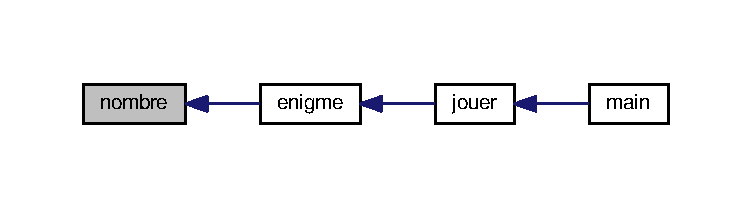
\includegraphics[width=350pt]{random_8c_a61c7a4ac34762307c8ad873e71774a43_icgraph}
\end{center}
\end{figure}



\hypertarget{random_8h}{}\section{Référence du fichier random.\+h}
\label{random_8h}\index{random.\+h@{random.\+h}}
Ce graphe montre quels fichiers incluent directement ou indirectement ce fichier \+:
\nopagebreak
\begin{figure}[H]
\begin{center}
\leavevmode
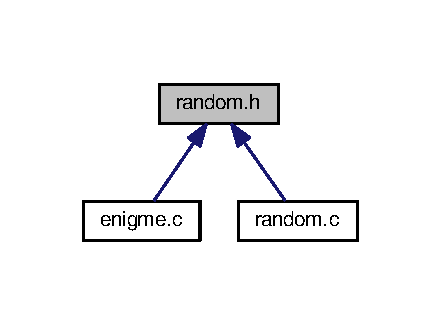
\includegraphics[width=212pt]{random_8h__dep__incl}
\end{center}
\end{figure}
\subsection*{Fonctions}
\begin{DoxyCompactItemize}
\item 
int \hyperlink{random_8h_a61c7a4ac34762307c8ad873e71774a43}{nombre} (void)
\begin{DoxyCompactList}\small\item\em Pour calculer un nbre aleatoire. \end{DoxyCompactList}\end{DoxyCompactItemize}


\subsection{Documentation des fonctions}
\index{random.\+h@{random.\+h}!nombre@{nombre}}
\index{nombre@{nombre}!random.\+h@{random.\+h}}
\subsubsection[{\texorpdfstring{nombre(void)}{nombre(void)}}]{\setlength{\rightskip}{0pt plus 5cm}int nombre (
\begin{DoxyParamCaption}
\item[{void}]{}
\end{DoxyParamCaption}
)}\hypertarget{random_8h_a61c7a4ac34762307c8ad873e71774a43}{}\label{random_8h_a61c7a4ac34762307c8ad873e71774a43}


Pour calculer un nbre aleatoire. 

\begin{DoxyAuthor}{Auteur}
Mintoua T Level-\/\+Up 
\end{DoxyAuthor}
\begin{DoxyDate}{Date}
Apr 28, 2019 
\end{DoxyDate}
\begin{DoxyReturn}{Renvoie}
un nbre 
\end{DoxyReturn}


Voici le graphe des appelants de cette fonction \+:
\nopagebreak
\begin{figure}[H]
\begin{center}
\leavevmode
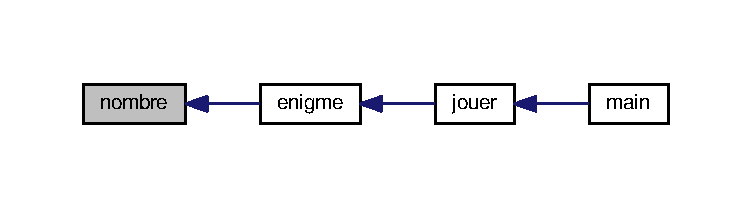
\includegraphics[width=350pt]{random_8h_a61c7a4ac34762307c8ad873e71774a43_icgraph}
\end{center}
\end{figure}



\hypertarget{text_8c}{}\section{Référence du fichier text.\+c}
\label{text_8c}\index{text.\+c@{text.\+c}}


Writing Program.  


{\ttfamily \#include \char`\"{}text.\+h\char`\"{}}\\*
{\ttfamily \#include \char`\"{}defs.\+h\char`\"{}}\\*
Graphe des dépendances par inclusion de text.\+c\+:\nopagebreak
\begin{figure}[H]
\begin{center}
\leavevmode
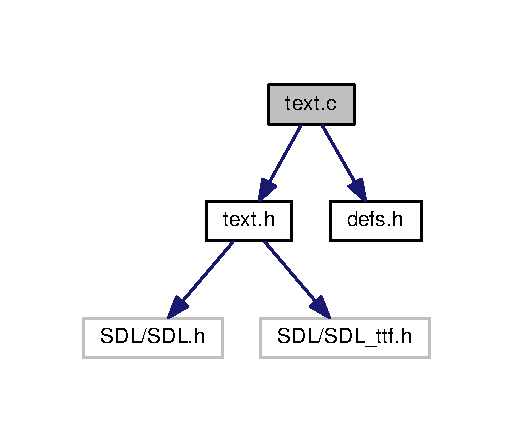
\includegraphics[width=246pt]{text_8c__incl}
\end{center}
\end{figure}
\subsection*{Fonctions}
\begin{DoxyCompactItemize}
\item 
void \hyperlink{text_8c_ab262a155d2f6fdeefc6ad6d63da93c82}{init\+Text} (\hyperlink{structText}{Text} $\ast$T)
\begin{DoxyCompactList}\small\item\em Pour Initialiser le texte. \end{DoxyCompactList}\item 
int \hyperlink{text_8c_a783bd5709ee569e182097ecc03ae9392}{load\+Font} (T\+T\+F\+\_\+\+Font $\ast$$\ast$police)
\begin{DoxyCompactList}\small\item\em Pour Charger le texte. \end{DoxyCompactList}\item 
void \hyperlink{text_8c_a6c91a76a6136671224fd357036b7e5b9}{display\+Text} (T\+T\+F\+\_\+\+Font $\ast$police, \hyperlink{structText}{Text} $\ast$T, S\+D\+L\+\_\+\+Surface $\ast$screen, int vie, int score, int tmp)
\begin{DoxyCompactList}\small\item\em Pour Afficher le texte. \end{DoxyCompactList}\item 
void \hyperlink{text_8c_aed94d72c6d43ac78f60f25e0d622d3bd}{free\+Font} (T\+T\+F\+\_\+\+Font $\ast$$\ast$police)
\begin{DoxyCompactList}\small\item\em Pour Liberer l\textquotesingle{}espace occupé par les textes. \end{DoxyCompactList}\end{DoxyCompactItemize}


\subsection{Description détaillée}
Writing Program. 

\begin{DoxyAuthor}{Auteur}
Mintoua T Level-\/\+Up 
\end{DoxyAuthor}
\begin{DoxyVersion}{Version}
0.\+1 
\end{DoxyVersion}
\begin{DoxyDate}{Date}
Apr 21, 2019
\end{DoxyDate}
Writing program for text 

\subsection{Documentation des fonctions}
\index{text.\+c@{text.\+c}!display\+Text@{display\+Text}}
\index{display\+Text@{display\+Text}!text.\+c@{text.\+c}}
\subsubsection[{\texorpdfstring{display\+Text(\+T\+T\+F\+\_\+\+Font $\ast$police, Text $\ast$\+T, S\+D\+L\+\_\+\+Surface $\ast$screen, int vie, int score, int tmp)}{displayText(TTF_Font *police, Text *T, SDL_Surface *screen, int vie, int score, int tmp)}}]{\setlength{\rightskip}{0pt plus 5cm}void display\+Text (
\begin{DoxyParamCaption}
\item[{T\+T\+F\+\_\+\+Font $\ast$}]{police, }
\item[{{\bf Text} $\ast$}]{T, }
\item[{S\+D\+L\+\_\+\+Surface $\ast$}]{screen, }
\item[{int}]{vie, }
\item[{int}]{score, }
\item[{int}]{tmp}
\end{DoxyParamCaption}
)}\hypertarget{text_8c_a6c91a76a6136671224fd357036b7e5b9}{}\label{text_8c_a6c91a76a6136671224fd357036b7e5b9}


Pour Afficher le texte. 

\begin{DoxyAuthor}{Auteur}
Mintoua T Level-\/\+Up 
\end{DoxyAuthor}

\begin{DoxyParams}{Paramètres}
{\em $\ast$police} & Le pointeur sur la police des textes \\
\hline
{\em $\ast$T} & Le texte ecrit \\
\hline
{\em screen} & Ecran du jeu \\
\hline
{\em vie} & vie joueur \\
\hline
{\em score} & son score \\
\hline
{\em tmp} & temps du jeu \\
\hline
\end{DoxyParams}
\begin{DoxyDate}{Date}
Apr 28, 2019 
\end{DoxyDate}
\begin{DoxyReturn}{Renvoie}
N\+U\+L\+L(rien) 
\end{DoxyReturn}


Voici le graphe des appelants de cette fonction \+:
\nopagebreak
\begin{figure}[H]
\begin{center}
\leavevmode
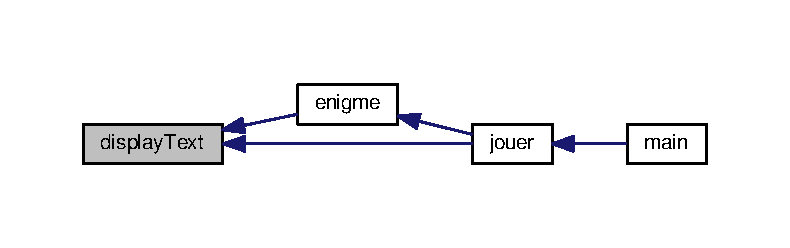
\includegraphics[width=350pt]{text_8c_a6c91a76a6136671224fd357036b7e5b9_icgraph}
\end{center}
\end{figure}


\index{text.\+c@{text.\+c}!free\+Font@{free\+Font}}
\index{free\+Font@{free\+Font}!text.\+c@{text.\+c}}
\subsubsection[{\texorpdfstring{free\+Font(\+T\+T\+F\+\_\+\+Font $\ast$$\ast$police)}{freeFont(TTF_Font **police)}}]{\setlength{\rightskip}{0pt plus 5cm}void free\+Font (
\begin{DoxyParamCaption}
\item[{T\+T\+F\+\_\+\+Font $\ast$$\ast$}]{police}
\end{DoxyParamCaption}
)}\hypertarget{text_8c_aed94d72c6d43ac78f60f25e0d622d3bd}{}\label{text_8c_aed94d72c6d43ac78f60f25e0d622d3bd}


Pour Liberer l\textquotesingle{}espace occupé par les textes. 

\begin{DoxyAuthor}{Auteur}
Mintoua T Level-\/\+Up 
\end{DoxyAuthor}

\begin{DoxyParams}{Paramètres}
{\em $\ast$police} & Le pointeur sur la police des textes \\
\hline
\end{DoxyParams}
\begin{DoxyDate}{Date}
Apr 28, 2019 
\end{DoxyDate}
\begin{DoxyReturn}{Renvoie}
N\+U\+L\+L(rien) 
\end{DoxyReturn}
\index{text.\+c@{text.\+c}!init\+Text@{init\+Text}}
\index{init\+Text@{init\+Text}!text.\+c@{text.\+c}}
\subsubsection[{\texorpdfstring{init\+Text(\+Text $\ast$\+T)}{initText(Text *T)}}]{\setlength{\rightskip}{0pt plus 5cm}void init\+Text (
\begin{DoxyParamCaption}
\item[{{\bf Text} $\ast$}]{T}
\end{DoxyParamCaption}
)}\hypertarget{text_8c_ab262a155d2f6fdeefc6ad6d63da93c82}{}\label{text_8c_ab262a155d2f6fdeefc6ad6d63da93c82}


Pour Initialiser le texte. 

\begin{DoxyAuthor}{Auteur}
Mintoua T Level-\/\+Up 
\end{DoxyAuthor}

\begin{DoxyParams}{Paramètres}
{\em T} & Le texte ecrit \\
\hline
\end{DoxyParams}
\begin{DoxyDate}{Date}
Apr 28, 2019 
\end{DoxyDate}
\begin{DoxyReturn}{Renvoie}
void(rien) 
\end{DoxyReturn}


Voici le graphe des appelants de cette fonction \+:
\nopagebreak
\begin{figure}[H]
\begin{center}
\leavevmode
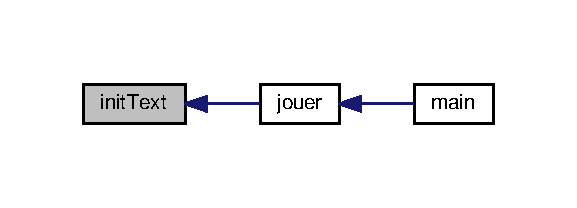
\includegraphics[width=277pt]{text_8c_ab262a155d2f6fdeefc6ad6d63da93c82_icgraph}
\end{center}
\end{figure}


\index{text.\+c@{text.\+c}!load\+Font@{load\+Font}}
\index{load\+Font@{load\+Font}!text.\+c@{text.\+c}}
\subsubsection[{\texorpdfstring{load\+Font(\+T\+T\+F\+\_\+\+Font $\ast$$\ast$police)}{loadFont(TTF_Font **police)}}]{\setlength{\rightskip}{0pt plus 5cm}int load\+Font (
\begin{DoxyParamCaption}
\item[{T\+T\+F\+\_\+\+Font $\ast$$\ast$}]{police}
\end{DoxyParamCaption}
)}\hypertarget{text_8c_a783bd5709ee569e182097ecc03ae9392}{}\label{text_8c_a783bd5709ee569e182097ecc03ae9392}


Pour Charger le texte. 

\begin{DoxyAuthor}{Auteur}
Mintoua T Level-\/\+Up 
\end{DoxyAuthor}

\begin{DoxyParams}{Paramètres}
{\em $\ast$police} & Le pointeur sur la police des textes \\
\hline
\end{DoxyParams}
\begin{DoxyDate}{Date}
Apr 28, 2019 
\end{DoxyDate}
\begin{DoxyReturn}{Renvoie}
E\+X\+I\+T\+\_\+\+F\+A\+I\+L\+U\+RE or E\+X\+I\+T\+\_\+\+S\+U\+C\+C\+E\+SS 
\end{DoxyReturn}


Voici le graphe des appelants de cette fonction \+:
\nopagebreak
\begin{figure}[H]
\begin{center}
\leavevmode
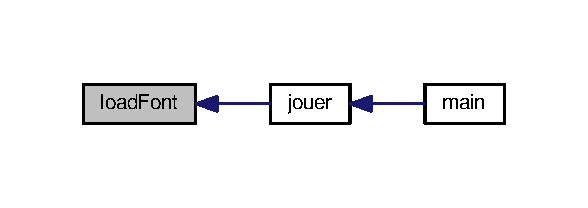
\includegraphics[width=282pt]{text_8c_a783bd5709ee569e182097ecc03ae9392_icgraph}
\end{center}
\end{figure}



\hypertarget{text_8h}{}\section{Référence du fichier text.\+h}
\label{text_8h}\index{text.\+h@{text.\+h}}
{\ttfamily \#include $<$S\+D\+L/\+S\+D\+L.\+h$>$}\\*
{\ttfamily \#include $<$S\+D\+L/\+S\+D\+L\+\_\+ttf.\+h$>$}\\*
Graphe des dépendances par inclusion de text.\+h\+:\nopagebreak
\begin{figure}[H]
\begin{center}
\leavevmode
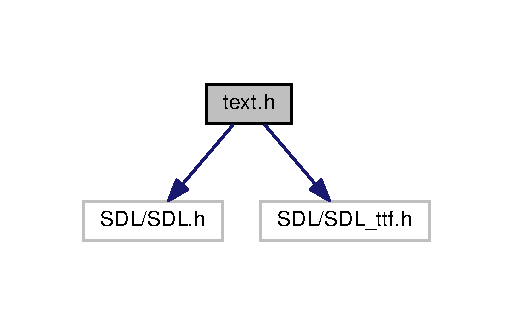
\includegraphics[width=246pt]{text_8h__incl}
\end{center}
\end{figure}
Ce graphe montre quels fichiers incluent directement ou indirectement ce fichier \+:
\nopagebreak
\begin{figure}[H]
\begin{center}
\leavevmode
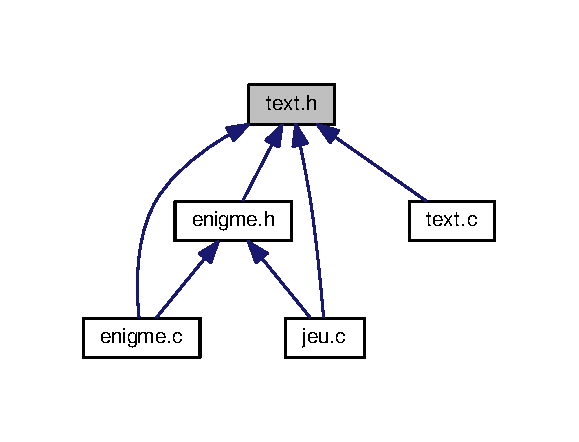
\includegraphics[width=278pt]{text_8h__dep__incl}
\end{center}
\end{figure}
\subsection*{Structures de données}
\begin{DoxyCompactItemize}
\item 
struct \hyperlink{structText}{Text}
\begin{DoxyCompactList}\small\item\em struct for \hyperlink{structText}{Text} \end{DoxyCompactList}\end{DoxyCompactItemize}
\subsection*{Définitions de type}
\begin{DoxyCompactItemize}
\item 
typedef struct \hyperlink{structText}{Text} \hyperlink{text_8h_a230d9bf1ae79368f80b618fa0e4eda09}{Text}
\end{DoxyCompactItemize}
\subsection*{Fonctions}
\begin{DoxyCompactItemize}
\item 
void \hyperlink{text_8h_ab262a155d2f6fdeefc6ad6d63da93c82}{init\+Text} (\hyperlink{structText}{Text} $\ast$T)
\begin{DoxyCompactList}\small\item\em Pour Initialiser le texte. \end{DoxyCompactList}\item 
int \hyperlink{text_8h_a783bd5709ee569e182097ecc03ae9392}{load\+Font} (T\+T\+F\+\_\+\+Font $\ast$$\ast$police)
\begin{DoxyCompactList}\small\item\em Pour Charger le texte. \end{DoxyCompactList}\item 
void \hyperlink{text_8h_a6c91a76a6136671224fd357036b7e5b9}{display\+Text} (T\+T\+F\+\_\+\+Font $\ast$police, \hyperlink{structText}{Text} $\ast$T, S\+D\+L\+\_\+\+Surface $\ast$screen, int vie, int score, int tmp)
\begin{DoxyCompactList}\small\item\em Pour Afficher le texte. \end{DoxyCompactList}\end{DoxyCompactItemize}


\subsection{Documentation des définitions de type}
\index{text.\+h@{text.\+h}!Text@{Text}}
\index{Text@{Text}!text.\+h@{text.\+h}}
\subsubsection[{\texorpdfstring{Text}{Text}}]{\setlength{\rightskip}{0pt plus 5cm}typedef struct {\bf Text} {\bf Text}}\hypertarget{text_8h_a230d9bf1ae79368f80b618fa0e4eda09}{}\label{text_8h_a230d9bf1ae79368f80b618fa0e4eda09}


\subsection{Documentation des fonctions}
\index{text.\+h@{text.\+h}!display\+Text@{display\+Text}}
\index{display\+Text@{display\+Text}!text.\+h@{text.\+h}}
\subsubsection[{\texorpdfstring{display\+Text(\+T\+T\+F\+\_\+\+Font $\ast$police, Text $\ast$\+T, S\+D\+L\+\_\+\+Surface $\ast$screen, int vie, int score, int tmp)}{displayText(TTF_Font *police, Text *T, SDL_Surface *screen, int vie, int score, int tmp)}}]{\setlength{\rightskip}{0pt plus 5cm}void display\+Text (
\begin{DoxyParamCaption}
\item[{T\+T\+F\+\_\+\+Font $\ast$}]{police, }
\item[{{\bf Text} $\ast$}]{T, }
\item[{S\+D\+L\+\_\+\+Surface $\ast$}]{screen, }
\item[{int}]{vie, }
\item[{int}]{score, }
\item[{int}]{tmp}
\end{DoxyParamCaption}
)}\hypertarget{text_8h_a6c91a76a6136671224fd357036b7e5b9}{}\label{text_8h_a6c91a76a6136671224fd357036b7e5b9}


Pour Afficher le texte. 

\begin{DoxyAuthor}{Auteur}
Mintoua T Level-\/\+Up 
\end{DoxyAuthor}

\begin{DoxyParams}{Paramètres}
{\em $\ast$police} & Le pointeur sur la police des textes \\
\hline
{\em $\ast$T} & Le texte ecrit \\
\hline
{\em screen} & Ecran du jeu \\
\hline
{\em vie} & vie joueur \\
\hline
{\em score} & son score \\
\hline
{\em tmp} & temps du jeu \\
\hline
\end{DoxyParams}
\begin{DoxyDate}{Date}
Apr 28, 2019 
\end{DoxyDate}
\begin{DoxyReturn}{Renvoie}
N\+U\+L\+L(rien) 
\end{DoxyReturn}


Voici le graphe des appelants de cette fonction \+:
\nopagebreak
\begin{figure}[H]
\begin{center}
\leavevmode
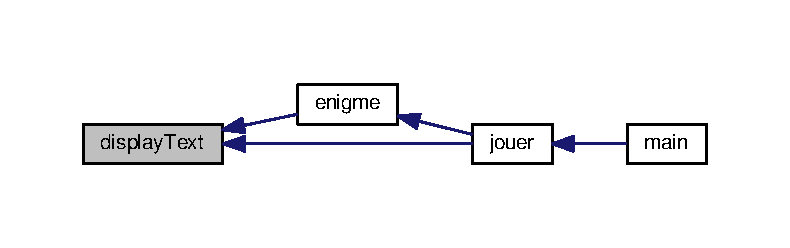
\includegraphics[width=350pt]{text_8h_a6c91a76a6136671224fd357036b7e5b9_icgraph}
\end{center}
\end{figure}


\index{text.\+h@{text.\+h}!init\+Text@{init\+Text}}
\index{init\+Text@{init\+Text}!text.\+h@{text.\+h}}
\subsubsection[{\texorpdfstring{init\+Text(\+Text $\ast$\+T)}{initText(Text *T)}}]{\setlength{\rightskip}{0pt plus 5cm}void init\+Text (
\begin{DoxyParamCaption}
\item[{{\bf Text} $\ast$}]{T}
\end{DoxyParamCaption}
)}\hypertarget{text_8h_ab262a155d2f6fdeefc6ad6d63da93c82}{}\label{text_8h_ab262a155d2f6fdeefc6ad6d63da93c82}


Pour Initialiser le texte. 

\begin{DoxyAuthor}{Auteur}
Mintoua T Level-\/\+Up 
\end{DoxyAuthor}

\begin{DoxyParams}{Paramètres}
{\em T} & Le texte ecrit \\
\hline
\end{DoxyParams}
\begin{DoxyDate}{Date}
Apr 28, 2019 
\end{DoxyDate}
\begin{DoxyReturn}{Renvoie}
void(rien) 
\end{DoxyReturn}


Voici le graphe des appelants de cette fonction \+:
\nopagebreak
\begin{figure}[H]
\begin{center}
\leavevmode
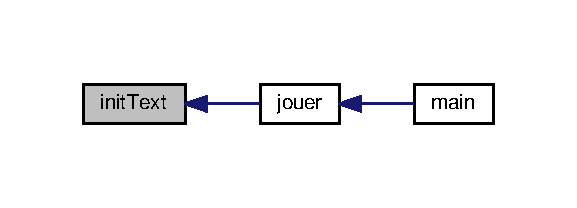
\includegraphics[width=277pt]{text_8h_ab262a155d2f6fdeefc6ad6d63da93c82_icgraph}
\end{center}
\end{figure}


\index{text.\+h@{text.\+h}!load\+Font@{load\+Font}}
\index{load\+Font@{load\+Font}!text.\+h@{text.\+h}}
\subsubsection[{\texorpdfstring{load\+Font(\+T\+T\+F\+\_\+\+Font $\ast$$\ast$police)}{loadFont(TTF_Font **police)}}]{\setlength{\rightskip}{0pt plus 5cm}int load\+Font (
\begin{DoxyParamCaption}
\item[{T\+T\+F\+\_\+\+Font $\ast$$\ast$}]{police}
\end{DoxyParamCaption}
)}\hypertarget{text_8h_a783bd5709ee569e182097ecc03ae9392}{}\label{text_8h_a783bd5709ee569e182097ecc03ae9392}


Pour Charger le texte. 

\begin{DoxyAuthor}{Auteur}
Mintoua T Level-\/\+Up 
\end{DoxyAuthor}

\begin{DoxyParams}{Paramètres}
{\em $\ast$police} & Le pointeur sur la police des textes \\
\hline
\end{DoxyParams}
\begin{DoxyDate}{Date}
Apr 28, 2019 
\end{DoxyDate}
\begin{DoxyReturn}{Renvoie}
E\+X\+I\+T\+\_\+\+F\+A\+I\+L\+U\+RE or E\+X\+I\+T\+\_\+\+S\+U\+C\+C\+E\+SS 
\end{DoxyReturn}


Voici le graphe des appelants de cette fonction \+:
\nopagebreak
\begin{figure}[H]
\begin{center}
\leavevmode
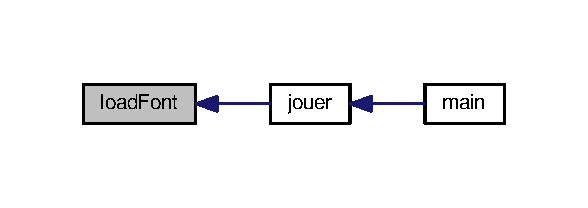
\includegraphics[width=282pt]{text_8h_a783bd5709ee569e182097ecc03ae9392_icgraph}
\end{center}
\end{figure}



%--- End generated contents ---

% Index
\backmatter
\newpage
\phantomsection
\clearemptydoublepage
\addcontentsline{toc}{chapter}{Index}
\printindex

\end{document}
